\documentclass[12pt]{article}
% \usepackage[top=1in,left=1in, right = 1in, footskip=1in]{geometry}
\usepackage[top=1in,footskip=1in]{geometry}

\usepackage{graphicx}
\usepackage{xspace}
%\usepackage{adjustbox}

\usepackage{multirow}
\usepackage{booktabs}

\usepackage{pdflscape}

\usepackage{grffile}

\newcommand{\comment}{\showcomment}
%% \newcommand{\comment}{\nocomment}

\newcommand{\showcomment}[3]{\textcolor{#1}{\textbf{[#2: }\textsl{#3}\textbf{]}}}
\newcommand{\nocomment}[3]{}

\newcommand{\jd}[1]{\comment{cyan}{JD}{#1}}
\newcommand{\swp}[1]{\comment{magenta}{SWP}{#1}}
\newcommand{\bmb}[1]{\comment{blue}{BMB}{#1}}
\newcommand{\djde}[1]{\comment{red}{DJDE}{#1}}

\newcommand{\eref}[1]{Eq.~(\ref{eq:#1})}
\newcommand{\fref}[1]{Fig.~\ref{fig:#1}}
\newcommand{\Fref}[1]{Fig.~\ref{fig:#1}}
\newcommand{\sref}[1]{Sec.~\ref{#1}}
\newcommand{\frange}[2]{Fig.~\ref{fig:#1}--\ref{fig:#2}}
\newcommand{\tref}[1]{Table~\ref{tab:#1}}
\newcommand{\tlab}[1]{\label{tab:#1}}
\newcommand{\seminar}{SE\mbox{$^m$}I\mbox{$^n$}R}

\usepackage{amsthm}
\usepackage{amsmath}
\usepackage{amssymb}
\usepackage{amsfonts}
\usepackage[utf8]{inputenc} % make sure fancy dashes etc. don't get dropped

\usepackage{lineno}
\linenumbers

\usepackage[pdfencoding=auto, psdextra]{hyperref}

\usepackage{natbib}
\bibliographystyle{chicago}
\date{\today}

\usepackage{xspace}
\newcommand*{\ie}{i.e.\@\xspace}

\usepackage{color}

\newcommand{\Rx}[1]{\ensuremath{{\mathcal R}_{#1}}\xspace} 
\newcommand{\RR}{\ensuremath{{\mathcal R}}\xspace}
\newcommand{\Rres}{\Rx{\mathrm{res}}}
\newcommand{\Rinv}{\Rx{\mathrm{inv}}}
\newcommand{\Rhat}{\ensuremath{{\hat\RR}}}
\newcommand{\Rt}{\ensuremath{{\mathcal R}(t)}\xspace}
\newcommand{\tsub}[2]{#1_{{\textrm{\tiny #2}}}}
\newcommand{\dd}[1]{\ensuremath{\, \mathrm{d}#1}}
\newcommand{\dtau}{\dd{\tau}}
\newcommand{\dx}{\dd{x}}
\newcommand{\dsigma}{\dd{\sigma}}

\newcommand{\rx}[1]{\ensuremath{{r}_{#1}}\xspace} 
\newcommand{\rres}{\rx{\mathrm{res}}}
\newcommand{\rinv}{\rx{\mathrm{inv}}}

\newcommand{\psymp}{\ensuremath{p}} %% primary symptom time
\newcommand{\ssymp}{\ensuremath{s}} %% secondary symptom time
\newcommand{\pinf}{\ensuremath{\alpha_1}} %% primary infection time
\newcommand{\sinf}{\ensuremath{\alpha_2}} %% secondary infection time

\newcommand{\psize}{{\mathcal P}} %% primary cohort size
\newcommand{\ssize}{{\mathcal S}} %% secondary cohort size

\newcommand{\gtime}{\tau_{\rm g}} %% generation interval
\newcommand{\gdist}{g} %% generation-interval distribution
\newcommand{\idist}{\ell} %% incubation-period distribution

\newcommand{\total}{{\mathcal T}} %% total number of serial intervals

\usepackage{lettrine}

\newcommand{\dropcapfont}{\fontfamily{lmss}\bfseries\fontsize{26pt}{28pt}\selectfont}
\newcommand{\dropcap}[1]{\lettrine[lines=2,lraise=0.05,findent=0.1em, nindent=0em]{{\dropcapfont{#1}}}{}}

\begin{document}

\begin{flushleft}{
	\Large
	\textbf\newline{
  Feasibility of using semi-mechanistic models for estimating long-term changes in infectious disease transmission from historical epidemic time series
	}
}
\newline
\\
Sang Woo Park\textsuperscript{1,*}, To be invited
\\
\bigskip
\textbf{1} School of Biological Sciences, Seoul National University, Seoul, Korea
\bigskip

*Corresponding author: sangwoopark@snu.ac.kr
\end{flushleft}

\section*{Abstract}

Understanding how disease transmission changes over time is a key challenge for predicting and preventing future outbreaks.
However, such efforts are often hampered by the many endogenous and exogenous factors that jointly affect transmission, including host immunity, demography, behavior, environmental conditions, and viral evolution.
Here, we developed a Bayesian semi-mechanistic approach for jointly estimating seasonal variation and flexible long-term changes in transmission without explicitly specifying these drivers.
An analysis of historical smallpox mortality data from London spanning more than 120 years suggested that considerable changes in transmission occurred over this period.
Simulation-recovery experiments demonstrated the feasibility of accurately estimating such changes, although small bias and improper uncertainty quantification remained an issue.
Allowing for time-varying reporting rate further illustrated that several major temporal features of the estimated trajectory can remain robust, although the magnitude and timing of some changes were sensitive to this assumption.
Further development of this framework could help test hypotheses about the drivers of long-term changes in disease transmission.

\pagebreak

\section*{Introduction}

A fundamental aim in infectious disease dynamics research is characterizing how disease transmission rates change over time \citep{grenfell2002dynamics,hooker2011parameterizing,becker2019long,jagan2020fast}.
For example, classic studies of endemic childhood infections, particularly measles, focused on estimating seasonal fluctuation in transmission rates driven by school term and climate effects \citep{fine1982measles,koelle2005refractory,ferrari2008dynamics,dalziel2016persistent}.
These efforts not only generated key insights into the drivers of epidemic dynamics but also established core methodological foundations for infectious disease research \citep{bjornstad2002dynamics,grenfell2002dynamics,he2010plug,king2016statistical}.
Yet transmission rates can also evolve over longer time scales, reflecting gradual shifts in host behavior \citep{weitz2020awareness,gozzi2025comparative}, demography, socioeconomic factors \citep{becker2019long}, and environmental conditions \citep{baker2019epidemic}.
Compared with seasonal variation, however, these low-frequency changes have received far less attention, in part because they are more difficult to identify from incidence data alone and are often confounded with other slow-moving processes such as susceptible replenishment and vaccination \citep{hooker2011parameterizing}.

Disruptions in disease transmission caused by COVID-19 nonpharmaceutical interventions also highlighted the similar need for new frameworks for estimating transmission rates that can vary flexibly across two different time scales:
explaining these disruptions requires simultaneous estimation of seasonal transmission patterns and rapid changes in transmission rate reflecting intervention effects.
To capture the impact of nonpharmaceutical interventions on disease transmission, some researchers have relied on known metrics of intervention strengths, such as mobility patterns \citep{park2024predicting2,howerton2025using} and stringency indices \citep{holmdahl2024differential,lau2024impact,yan2026impact}, whereas other have sought to directly estimate these impacts through various statistical methods \citep{flaxman2020estimating,bents2023modeling,sauteur2025global,nguyen2026dynamics}.
Notably, models utilizing Bayesian inference framework have proven particularly useful for estimating flexible changes in transmission patterns, where statistical constraints through prior distributions can appropriately limit the variability in parameter estimates \citep{flaxman2020estimating,park2024predicting,nielsen2025complex,park2025interplay}.
These methodological advances provide a basis for developing semi-mechanistic models that allow estimation of transmission rates across two different time scales, with potential applications beyond the context of COVID-19 interventions, but their estimability and generalizability have not yet been tested.
Furthermore, the apparent discrepancy between the estimated intervention effects and observed changes in mobility patterns indicate potential challenges in interpreting parameter estimates from semi-mechanistic models \citep{park2024predicting}.

Inspired by these efforts, we present a Bayesian semi-mechanistic framework for simultaneously estimating seasonal and long-term variation in disease transmission and investigate its estimability and interpretibility.
We test the resulting framework against a 126-year long time series of smallpox deaths, which presents a computationally challenging example.
We then validate the methodology using simulation-recovery experiments.

\section*{Results}

\subsection*{Developing semi-mechanistic models for estimating seasonal and long-term variation in disease transmission}

\begin{figure}[!ht]
\begin{center}
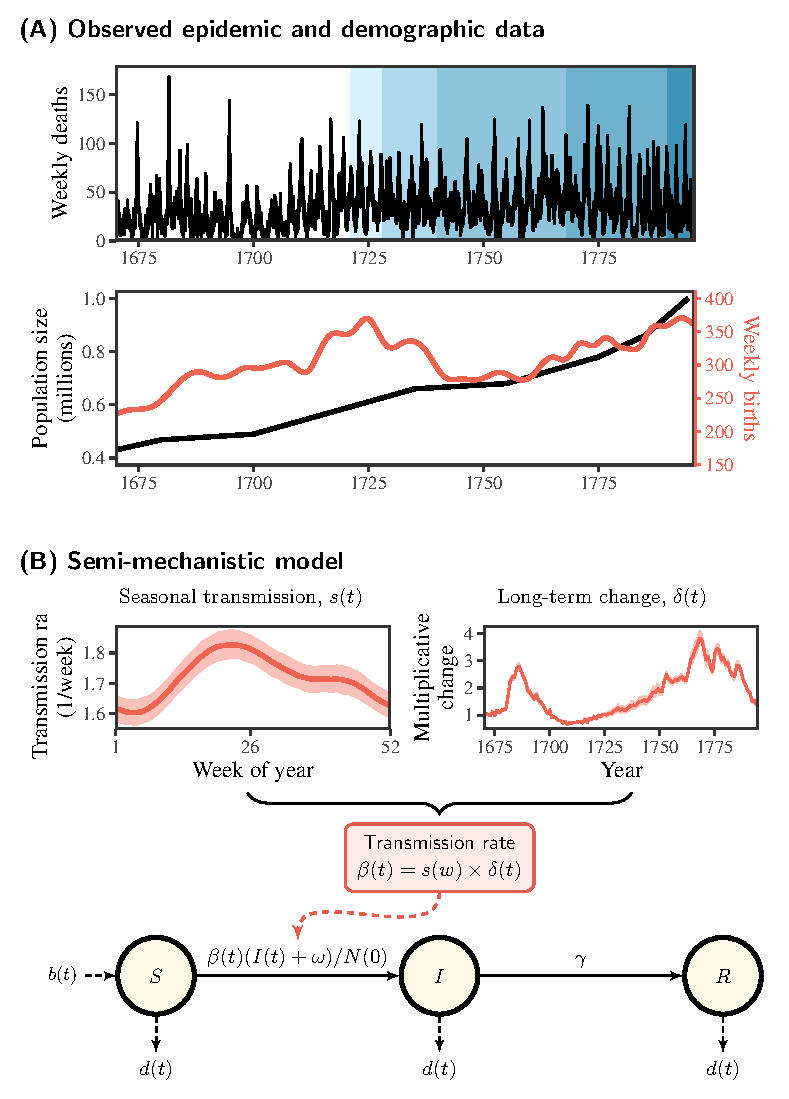
\includegraphics[width=0.8\textwidth]{../diagram_model/diagram_model.pdf}
\caption{
\textbf{Developing semi-mechanistic models for estimating long-term changes in transmission from historical epidemic time series data.}
(A) Observed epidemic and demographic data, including population size and birth rate.
Blue shaded regions indicate the increasing intensity of variolation practices.
(B) Schematic diagram illustrating the semi-mechanistic model.
The semi-mechanistic model allows for slow, annual variation and fast, seasonal variation in disease transmission rates.
}
\end{center}
\end{figure}

First, the data set consisted of weekly reports of smallpox deaths spanning 126 years (Figure 1A).
During this period, many factors that could affect disease transmission changed, including variolation practices and demographic patterns.
For instance, variolation was first introduced in 1721 and increased in intensity until the late 1790s and early 1800s, when vaccination was introduced.
These changes likely decreased smallpox transmission, but quantifying the prevalence and effectiveness of variolation practices is challenging.
During the same period, the birth rate also increased, contributing to an almost 2.5-fold increase in population size, which likely increased contact rates and smallpox transmission.
Many other changes likely occurred, including changes in sanitary practices and population structure.

It would be infeasible to explicitly incorporate all these changes into a model, especially because quantitative data describing the underlying changes are unavailable.
Instead, our goal was to develop a semi-mechanistic model that seeks to implicitly capture the effects of unmodeled factors on disease transmission (Figure 1B).
Specifically, we decomposed the transmission rate $\beta(t)$ of the classic SIR model into a seasonal term $\tsub{\beta}{seas}(t)$ and a slow, time-varying term $\delta(t)$:
\begin{equation}
\beta(t) = \frac{\tsub{\beta}{seas}(t) \delta(t)}{N_{1670}},
\end{equation}
where $N_{1670}$ represents the population size at the beginning of 1670, which is included to scale the $\tsub{\beta}{seas}(t)$.
Here, dependence transmission is assumed to account for potential impact of increase in population sizes on transmission.
The time-varying term $\delta(t)$ was allowed to vary every year.
Both $\tsub{\beta}{seas}(t)$ and $\delta(t)$ terms were modeled using random walk priors to impose smoothness.
We then try to fit the resulting SIR model to the time series of smallpox deaths and try to estimate both terms simultaneously using Bayesian inference.

Fitting the resulting model to 126 years of weekly observations presents substantial computational challenges. 
To address these challenges, we obtained maximum a posteriori estimates through optimization and used a Laplace approximation to characterize posterior uncertainty.
Implementation details are provided in the Materials and Methods section.

\subsection*{Potential long-term changes in smallpox transmission}

\begin{figure}[!ht]
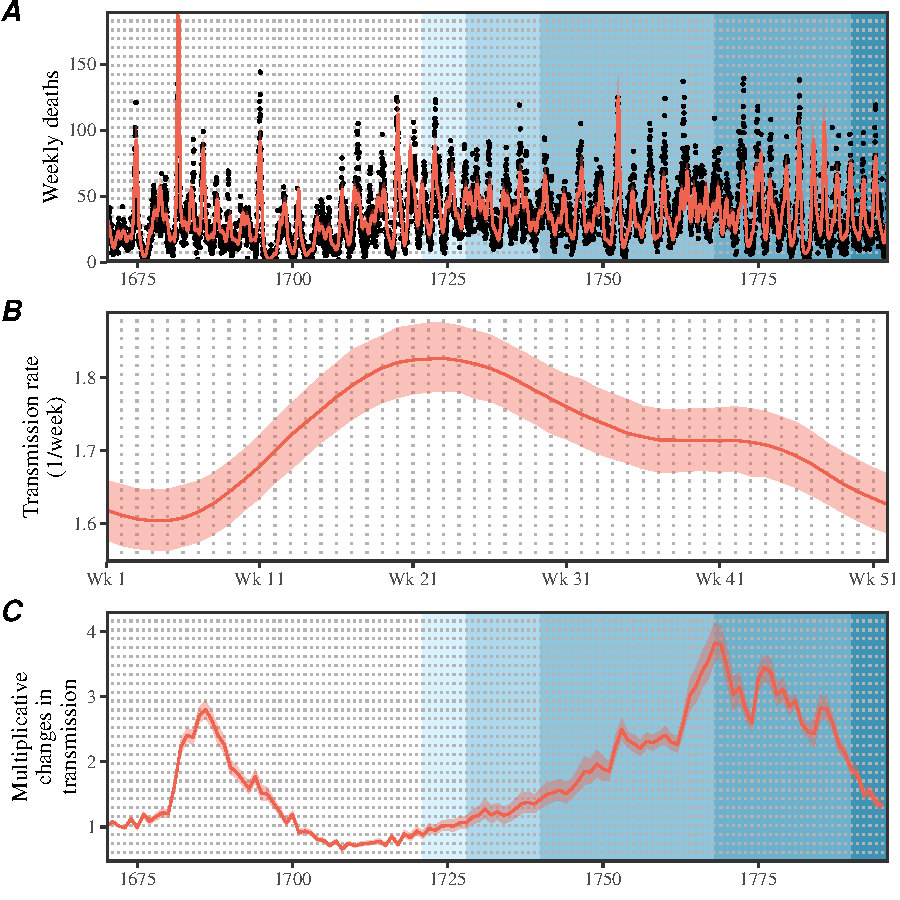
\includegraphics[width=\textwidth]{../figure/figure_stanfit.pdf}
\caption{
\textbf{Summary of model fits to smallpox data set.}
(A) Observed data (black points) and model fits (red lines).
(B) Estimated seasonal transmission rate.
(C) Estimated multiplicative changes in annual transmission.
Red lines indicate the posterior median estimate and shaded regions represent the 90\% credible interval.
Blue shaded regions indicate the increasing intensity of variolation practices.
}
\end{figure}

Our semi-mechanistic SIR model was able to capture the overall epidemic patterns across the 126-year time series, including long-term changes in outbreak magnitude (Figure 2A).
In particular, we estimated a clear seasonal pattern in transmission, with transmission increasing from the beginning of the year, peaking around week 23, and then gradually decreasing toward the end of the year (Figure 2B).

We also estimated substantial long-term variation in transmission rates (Figure 2C).
The annual transmission term increased sharply during the 1680s, reaching nearly three times its value in 1670, and then declined to its lowest value around early 1700s.
Even after the introduction of variolation in 1721, the annual transmission multiplier gradually increased again, reaching almost four times its 1670 value in the late 1760s.
Despite the continued increase in the intensity of variolation practices, annual transmission remained relatively high throughout the 1770s and 1780s before decreasing rapidly toward the end of the study period.
This apparent discrepancy suggests that the estimated annual transmission term likely captures the combined effects of multiple unmodeled factors rather than the effect of variolation alone.

\subsection*{Simulation-recovery experiments}

\begin{figure}[!ht]
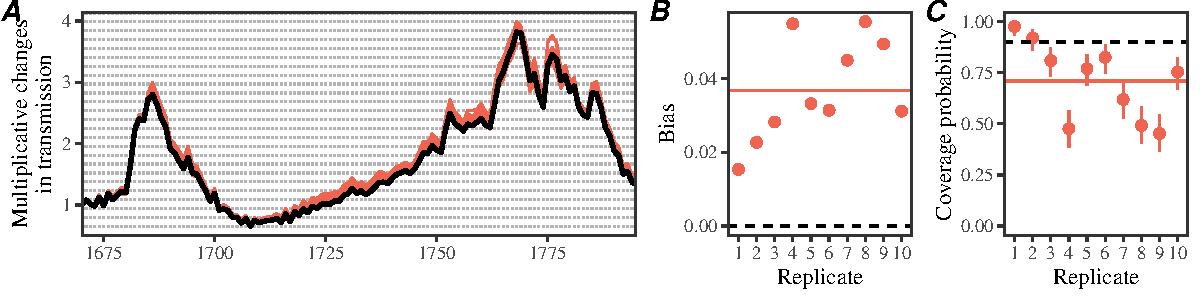
\includegraphics[width=\textwidth]{../figure_rep/figure_stanfit_rep.pdf}
\caption{
\textbf{Summary of simulation-recovery experiments.}
(A) Comparisons between the assumed (black) and estimated (red) changes in annual transmission rates.
(B) Mean bias across estimated changes in annual transmission rates for each replicates.
The black dashed line represents zero bias.
The red line represents the average value across replicates.
(C) Mean coverage probability across estimated changes in annual transmission rates for each replicates.
The black dashed line represents the nominal coverage probability (0.9).
The red line represents the average value across replicates.
}
\end{figure}

The discrepancy between increasing variolation efforts, which we expected to drive reduction in transmission, and the estimated patterns of increasing transmission further raises a question of whether the semi-mechanistic model is able to correctly estimate the underlying transmission pattern.
Thus, we performed simulation recovery experiments, where we generated 10 synthetic time series using the estimated values and fitted the same model to each time series independently (Figure 3).
We found that our model is able to accurately recover long-term changes in transmission (Figure 3A).
Across all 10 simulations, the model was able to accurately capture the observed epidemic patterns with $R^2$ values over 0.7 consistently.
However, our methodology introduced some bias ($\approx 4\%$; Figure 3B) and provided low coverage values ($\approx 0.7$; Figure 3C), suggesting overly narrow credible intervals.  

\begin{figure}[!ht]
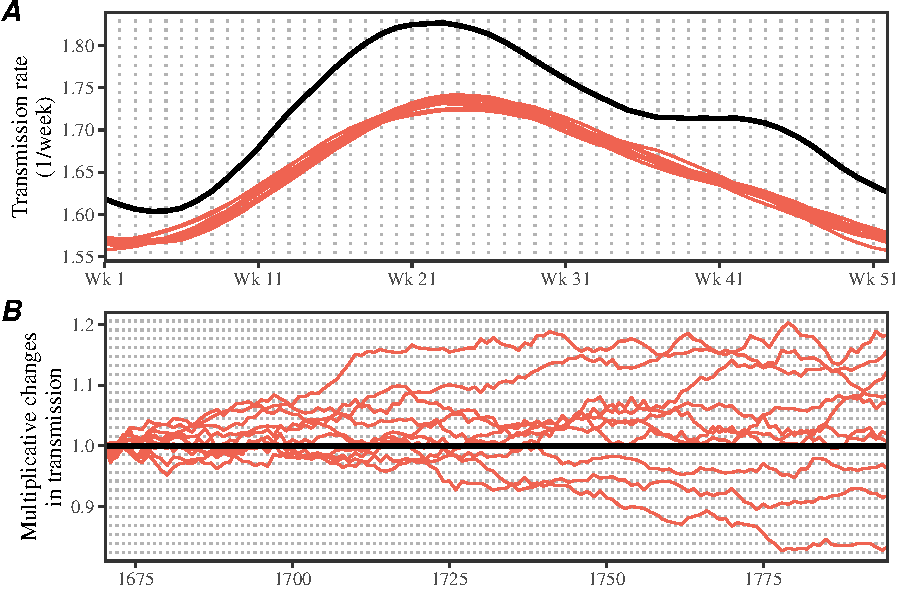
\includegraphics[width=\textwidth]{../figure_rep_nc/figure_stanfit_rep_nc.pdf}
\caption{
\textbf{Summary of simulation-recovery experiments in the absence of long-term changes in transmission.}
(A) Comparisons between the assumed (black) and estimated (red) changes in annual transmission rates.
(B) Mean bias across estimated changes in annual transmission rates for each replicates.
The black dashed line represents zero bias.
The red line represents the average value across replicates.
(C) Mean coverage probability across estimated changes in annual transmission rates for each replicates.
The black dashed line represents the nominal coverage probability (0.9).
The red line represents the average value across replicates.
}
\end{figure}

As a negative control experiment, we also generated 10 synthetic time series, where the annual term $\delta(t)$ is set to 1, and fit the same model to each time series independently (Figure 4).
Since we assumed random walk priors, the estimated long-term changes in transmission diverged from one, leading up to 20\% estimated changes in transmission rates over 126 years (Figure 4A).
Despite this divergence, our estimates still did not generate any meaningful patterns and provided high coverage values ($\approx 1$), indicating that credible intervals consistently includes one and that deviation from one is not statistically meaningful (Figure 4C). 
For this experiment, the model also gave similar but slightly smaller levels of bias ($\approx 2\%$; Figure 4B).

\subsection*{Changes in reporting rate}


\begin{figure}[!ht]
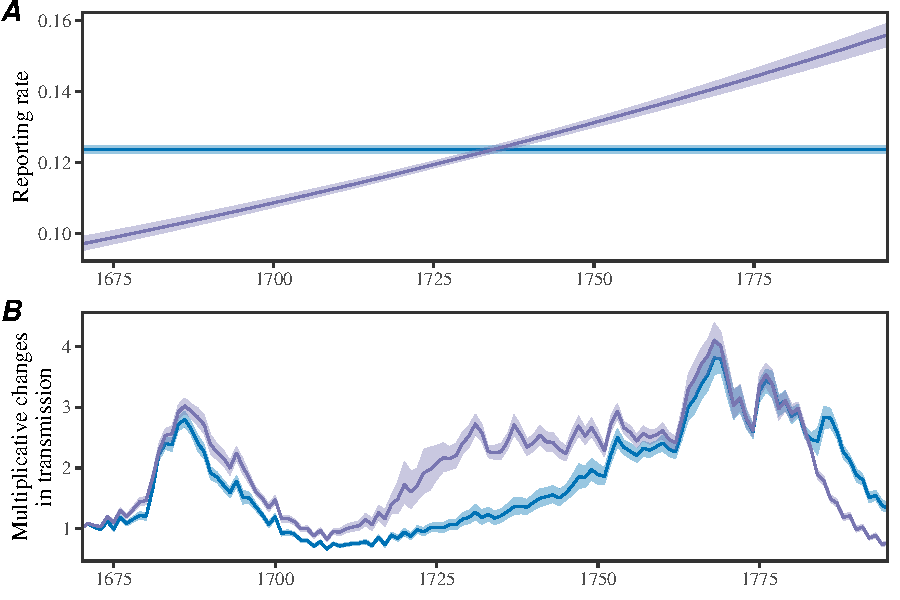
\includegraphics[width=\textwidth]{../figure/figure_stanfit_rho.pdf}
\caption{
\textbf{Estimated reporting rates and corresponding long-term changes in transmission.}
(A) Estimated reporting rates assuming constant (red) and exponentially changing (blue) reporting rates.
(B) Estimated multiplicative changes in annual transmission.
Colored lines indicate posterior median estimates and shaded regions represent 90\% credible intervals.
}
\end{figure}

So far, we assumed a fixed reporting rate throughout the entire study period, which was estimated to be around 12.4\% (90\% CI: 12.3\%--12.5\%) (Figure 5A).
However, it is unlikely for reporting rate to stay constant over a such long period of time.
To test the effect of changing reporting rates in our estimates of long-term changes in transmission, we allowed the reporting rate to change exponentially over time and refitted the model.
Under this assumption, we estimated the reporting rate to increase from 9.7\% to 15.6\% over 126 years, corresponding to a 1.6 fold increase (Figure 5A).
Qualitative patterns in in the estimated long-term transmission rate remained robust (e.g., increase in transmission from the early 1700s to 1770s and a decrease in transmission in the late 1780s), but the exact values differ substantially from our initial estimates based on fixed reporting rate (Figure 5B).

\section*{Discussion}

Here, we developed a Bayesian semi-mechanistic approach for estimating long-term changes in transmission from epidemic time series.
We demonstrated its application using historical smallpox mortality data spanning more than 120 years and evaluated its performance using simulation-recovery experiments. 
These experiments demonstrated that the approach can accurately recover broad changes in transmission under the assumed model.
Allowing reporting rates to vary over time preserved several major temporal features of the estimated transmission trajectory, but altered the magnitude and timing of some changes, highlighting both the robustness of these features and the sensitivity of the reconstruction to underlying model assumptions.

Our study builds on earlier efforts to reconstruct transmission from long epidemic time series by estimating flexible long-term changes within a Bayesian semi-mechanistic framework.
The most relevant precedent is \cite{krylova2011predicting}, who extended the approach of \cite{fine1982measles} to reconstruct smallpox transmission in London from 1664 to 1930. 
This analysis focused on changes in seasonal transmission patterns, but also identified an increase in mean transmission between the 1660s and 1760s;
we note that the degree of increase was considerably smaller than ours.
These changes were summarized by averaging across distinct historical periods, whereas our framework explicitly estimates a long-term transmission trajectory and its associated uncertainty.
Another close precedent is \cite{becker2019long}, who fitted an SEIR model to measles mortality and incidence data from London between 1897 and 1991. 
Interestingly, they found that most changes in epidemic dynamics could be explained by changes in demography and vaccination under a fixed seasonal transmission pattern, with additional perturbations associated with the 1918 influenza pandemic and World War II.
Over a shorter period, \cite{hooker2011parameterizing} estimated a linear increase in transmission from Ontario measles data spanning 1939–1965, although this trend was highly uncertain. 
To our knowledge, this is the first study to jointly reconstruct seasonal variation and flexible long-term changes in transmission within a Bayesian framework from an epidemic time series spanning more than a century.

There are several limitations to our framework, which suggest new directions for future methodological development.
First of all, fitting a semi-mechanistic model to such long time series using Markov Chain Monte Carlo can be computationally intensive.
To remedy this issue, we relied on simple optimization and a Laplace approximation to obtain an approximate posterior.
However, full Monte Carlo sampling is needed to assess whether this approximation accurately captures posterior uncertainty.
Indeed, we found that the current framework can introduce a small amount of bias and provide overly narrow or wide credible intervals, depending on the scenario.
Other approximations, such as variational inference, can also be explored.

Second, our reporting rate anlysis indicates that the exact transmission trajectory can be sensitive to unedrlying model assumptions.
Here, we focused on simple sensitivity analysis to demonstrate that some temporal patterns can still remain robust, but exhaustive modeling effort is needed to assess which of the estimated patterns are real signals, rather than statistical artifacts.
Thus, while our analysis suggested considerable changes in transmission patterns over the century, we caution against assigning biological interpretations to these changes without additional evidence.

Finally, identifying the drivers of the estimated transmission trajectory remains a significant challenge for semi-mechanistic models.
Even when temporal patterns are robust to model assumptions, their underlying causes may remain unclear.
Such efforts would require detailed data on behavioral and demographic changes over the course of the epidemic, but gathering these data can be particularly challenging for historical epidemics.
Even when available, these data may not be sufficient to explain the estimated changes in transmission.
For example, \cite{park2024predicting} noted that estimated changes in transmission of \textit{Mycoplasma pneumoniae} during the COVID-19 pandemic did not correlate with observed mobility patterns.
Future work should consider incorporating candidate drivers directly into the transmission model alongside flexible terms that capture unexplained variation.
Despite these limitations, our analysis offers a methodological advancement from current modeling approaches, demonstrating the feasibility of jointly estimating long-term changes in transmission and seasonal variation from an epidemic time series spanning more than a century.

In conclusion, semi-mechanistic models offer a flexible approach for estimating transmission trajectories without explicitly specifying their drivers.
While several limitations remain, this framework provides a starting point for investigating changes in transmission across different timescales.
Further development of these approaches could help use long epidemic records to generate and test hypotheses about the mechanisms underlying changes in disease dynamics.

\section*{Materials and Methods}

\subsection*{Data}

We used a weekly time series of smallpox deaths to test the ability of a semi-mechanistic model to infer long-term changes in disease transmission (Figure 1).
The original data set spans from 1664 to 1930 and was digitized from London Bills of Mortality and the Registrar General’s Weekly Returns by \cite{krylova2020patterns}.
Here, we considered mortality records between 1670 and 1795 to focus on the dynamics before the discovery of vaccination.
Even in the absence of vaccination, an increase in variolation to protect against severe outcomes (Figure 1A) and a rapid increase in population sizes due to increasing births (Figure 1B,C) would have caused complex changes in transmission conditions over the 126-year period, which cannot be explained by traditional modeling approaches that only account for seasonal transmission forcing. 
Data on population sizes and birth rates were obtained from the publicly available data set from \citep{krylova2020patterns}.
Death rates were calculated to match increasing rates of population sizes:
specifically, we calculated the difference between the weekly rate of population size increase and weekly  birth rate to obtain weekly death rates.

\subsection*{Mathematical model}

To focus on the feasibility of estimating long-term changes in transmission, we decided to use the simplest transmission model, namely the SIR model.
Assuming density dependent transmission, the discrete time SIR model can be written as:
\begin{align}
\mathrm{FOI}(t) &= \beta(t) (I(t) + \omega) \\
\Delta S(t) &= \left[1- \exp(-(\mathrm{FOI}(t) + d(t)) \Delta t )\right] S(t-\Delta t)\\
N_{SI}(t) &= \frac{\mathrm{FOI}(t)\Delta S(t)}{\mathrm{FOI}(t) + d(t)} \\
\Delta I(t) &= \left[1- \exp(-(\gamma + d(t)) \Delta t )\right] I(t-\Delta t)\\
N_{IR}(t) &= \frac{\gamma \Delta I(t)}{\gamma + d(t)} \\
S(t) &= S(t-\Delta t) + b(t) N - \Delta S(t) \\
I(t) &= I(t-\Delta t) - \Delta I(t) + N_{SI}(t)
\end{align}
where $\mathrm{FOI}(t)$ represents the force of infection;
$\beta(t)$ represents the transmission rate;
$\omega$ represents the number of imported infections;
$\gamma$ represents the recovery rate;
$d(t)$ represents the death rate;
and $b(t)$ represents the birth rate.
The transmission rate is decomposed into a seasonal term $\tsub{\beta}{seas}(t)$ and a multiplicative time-varying transmission term $\delta(t)$:
\begin{equation}
\beta(t) = \frac{\tsub{\beta}{seas}(t) \delta(t)}{N_{1670}},
\end{equation}
where $N_{1670}$ represents the population size at the beginning of 1670, which is included to scale the $\tsub{\beta}{seas}(t)$.
Previous studies have illustrated the feasibility of estimating $\delta(t)$ at different time scales by anchoring the seasonal term $\tsub{\beta}{seas}(t)$ to certain periods.
For example, when inferring the impact of COVID-19 interventions, $\delta(t)$ was set to 1 during the pre-pandemic period and allowed to vary from 2020 onward, with change points defined at intervals ranging from one to four weeks \citep{park2024predicting,nielsen2025complex,park2025interplay}.
Since we are interested in capturing long-term changes in transmission, we allowed $\delta(t)$ to vary every year.

\subsection*{Statistical inference and implementation}

In order to simultaneously estimate $\tsub{\beta}{seas}(t)$ and $\delta(t)$ alongside other parameters and initial conditions, we needed to appropriately constrain the parameter space.
Otherwise, estimating 52 terms for $\tsub{\beta}{seas}(t)$ and 126 terms for $\delta(t)$ would require estimation of $>170$ parameters, which is more than an order of magnitude greater than the number of parameters that are estimated for a typical infectious disease model.
Bayesian inference, implemented via the Stan software, enables us to constrain the parameter space through prior distributions and allows for fast, efficient inference through state-of-art inference algorithms \citep{carpenter2017stan}. 
We first discuss our model parameterization, prior choices, and observation models used for fitting.
Then, we describe our implementation in Stan.

If we were to estimate all 52 terms of the seasonal term $\tsub{\beta}{seas}(t)$ separately, then the resulting transmission rate may not be realistic and difficult to interpret.
Thus, to constrain the shape of the seasonal term $\tsub{\beta}{seas}(t)$ and allow for biological interpretation, we imposed a cyclic, random-walk prior on a log scale \citep{park2025interplay}:
\begin{align}
\log\tsub{\beta}{seas}(t+1) &\sim \mathrm{Normal}(\log\tsub{\beta}{seas}(t), \tsub{\sigma}{seas}), \quad t=1,\dots,51  \\
\log\tsub{\beta}{seas}(1) &\sim \mathrm{Normal}(\log\tsub{\beta}{seas}(52), \tsub{\sigma}{seas})
\end{align}
where the standard deviation $\tsub{\sigma}{seas}$ determines the smoothness of the seasonal transmission rate.
Strong priors were imposed to constrain the parameter space for $\tsub{\sigma}{seas}$:
\begin{equation}
\tsub{\sigma}{seas} \sim \textrm{Half-Normal}(0, 0.01).
\end{equation}
We further imposed an informative prior on $\tsub{\beta}{seas}(t)$, reflecting previously reported $\mathcal R_0$ values for smallpox transmission:
\begin{equation}
\log\tsub{\beta}{seas}(t) \sim \mathrm{Normal}(0.5, 0.1).
\end{equation}
Combined with the assumed recovery rate of $-\log(1-1/3)/\mathrm{weeks}$, which corresponds to a mean infectious period of 3 weeks, the prior distribution of the basic reproduction number has a median of 4.9 and a 95\% quantile of 4.1 to 6.0.

For similar reasons as above, we also utilized random walk priors to model the multiplicative time-varying transmission term on a log scale: $\delta(t) = \exp(\epsilon(t))$.
In order to reduce correlations in posterior distributions, we parameterized $\epsilon(t)$ by expression it as a sum of independent normal variables $z_\epsilon(t)$:
\begin{align}
z_\epsilon(t) &\sim \mathrm{Normal}(0, 1), \quad t = 1671, \dots, 1795 \\
\sigma_\epsilon &\sim \textrm{Half-Normal}(0, 0.01)\\
\epsilon(1670) &= 0\\
\epsilon(t) &= \epsilon(t-1) + \sigma_\epsilon z_\epsilon, \quad t = 1671, \dots, 1795 \\
\delta(t) &= \exp(\epsilon(t))
\end{align}
where $z_\epsilon(t)$ determines the smoothness of $\epsilon(t)$. By setting the initial $\epsilon(1670)$ to zero and imposing constraining priors on $\sigma_\epsilon$, this approach anchors the seasonal transmission term $\tsub{\beta}{seas}(t)$ to early periods and allow for slow variation in transmission rates over time.

The model was fitted to smallpox deaths $D(t)$ by assuming a negative binomial observation model:
\begin{align}
D(t) &\sim \textrm{NegBin}(\rho N_{IR}(t), \phi)\\
\rho &\sim \textrm{Beta}(1,1)\\
\phi &\sim \textrm{Normal}(100, 20)
\end{align}
where $\rho$ represents the infection mortality rate, and $\phi$ represents the overdispersion parameter.
Alongside parameters described earlier, we also estimated the initial conditions $S(1670)$ and $I(1670)$ at the beginning of 1670 as well as imported infections $\omega$:
\begin{align}
S(1670) &\sim \textrm{Beta}(1, 1)\\
I(1670) &\sim \textrm{Half-Normal}(0,0.001)\\
\omega &\sim \textrm{Half-Normal}(0, 200)
\end{align}

Previous studies primarily relied on Hamiltonian Monte Carlo (HMC) sampling implemented in Stan to estimate parameters of transmission models \citep{park2024predicting,nielsen2025complex,park2025interplay}.
While this approach enables efficient exploration of high-dimensional parameter spaces and provides accurate uncertainty quantification, inference can remain computationally demanding for nonlinear models with many parameters. 
During our investigation, we also encountered convergence issues, partly reflecting the sensitivity of HMC sampling to initial conditions.
Instead, we began with an optimization from 100 random starting values to obtain the maximum a posteriori estimates.
Then, we used Laplace approximation to obtain approximate posterior distributions.

\subsection*{Simulation studies}

To evaluate the ability of a semi-mechanistic model to correctly infer seasonal and long-term variation in transmission rates, we generated a synthetic data set using median posterior estimates from the smallpox analysis.
We then fitted the same model using the same process as outlined above, using 100 random starting values for optimization.
We repeated the analysis 10 times.

As a negative control, we also simulated the model without long-term changes in transmission rates, thus fixing $\epsilon = 0$. 
We then fitted the same model using the same process as outlined above, using 100 random starting values for optimization, repeating the analysis 10 times.
For both simulation studies, we compute relative bias and coverage probabilities (using 90\% credible interval) for the estimated long-term changes in transmission.

\pagebreak

\renewcommand\theequation{S\arabic{equation}}
\renewcommand\thefigure{S\arabic{figure}}    
\setcounter{equation}{0}
\setcounter{figure}{0}

\section*{Supplementary Figure}

\begin{figure}[!ht]
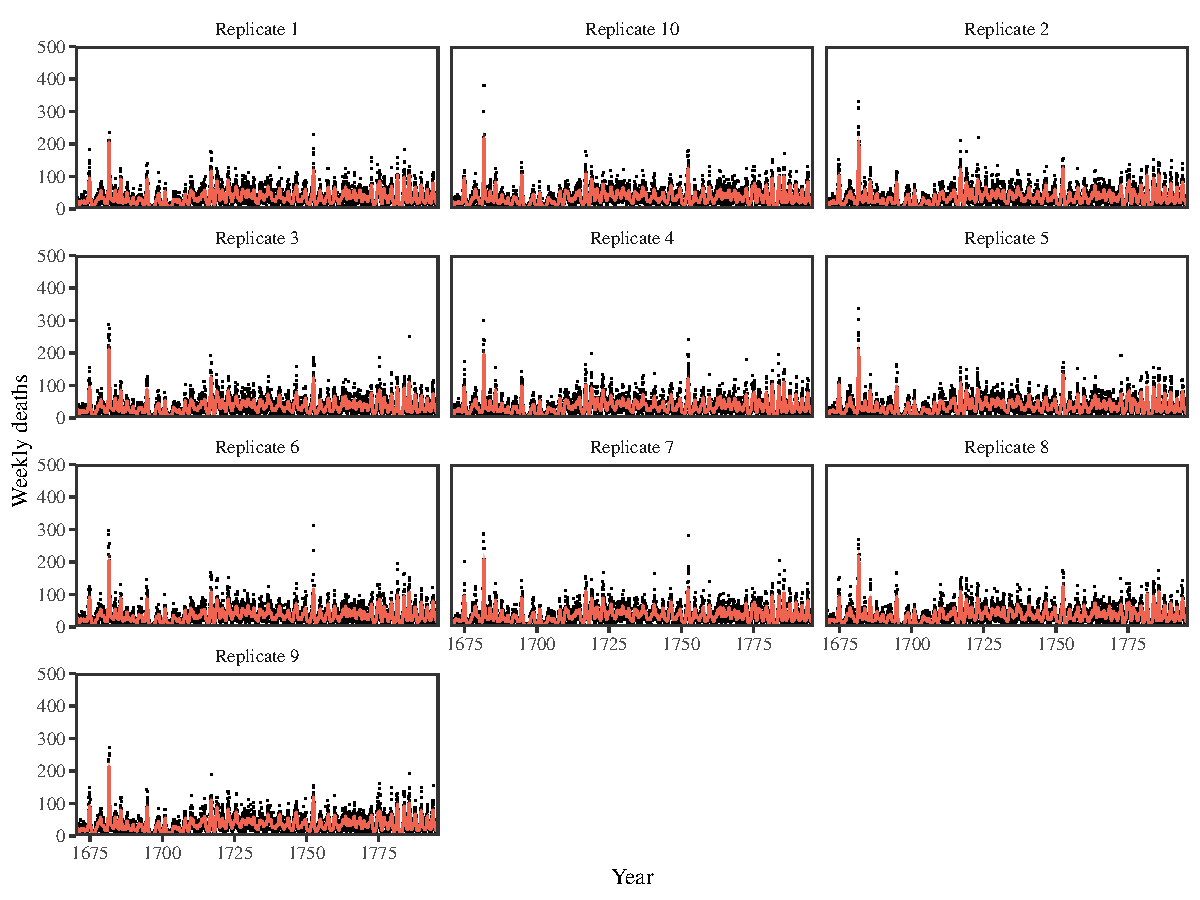
\includegraphics[width=\textwidth]{../figure_rep/figure_stanfit_rep_traj_1.pdf}
\caption{
\textbf{Comparisons between observed and predicted epidemic trajectories from simulation recovery experiments.}
}
\end{figure}

\pagebreak


\begin{figure}[!ht]
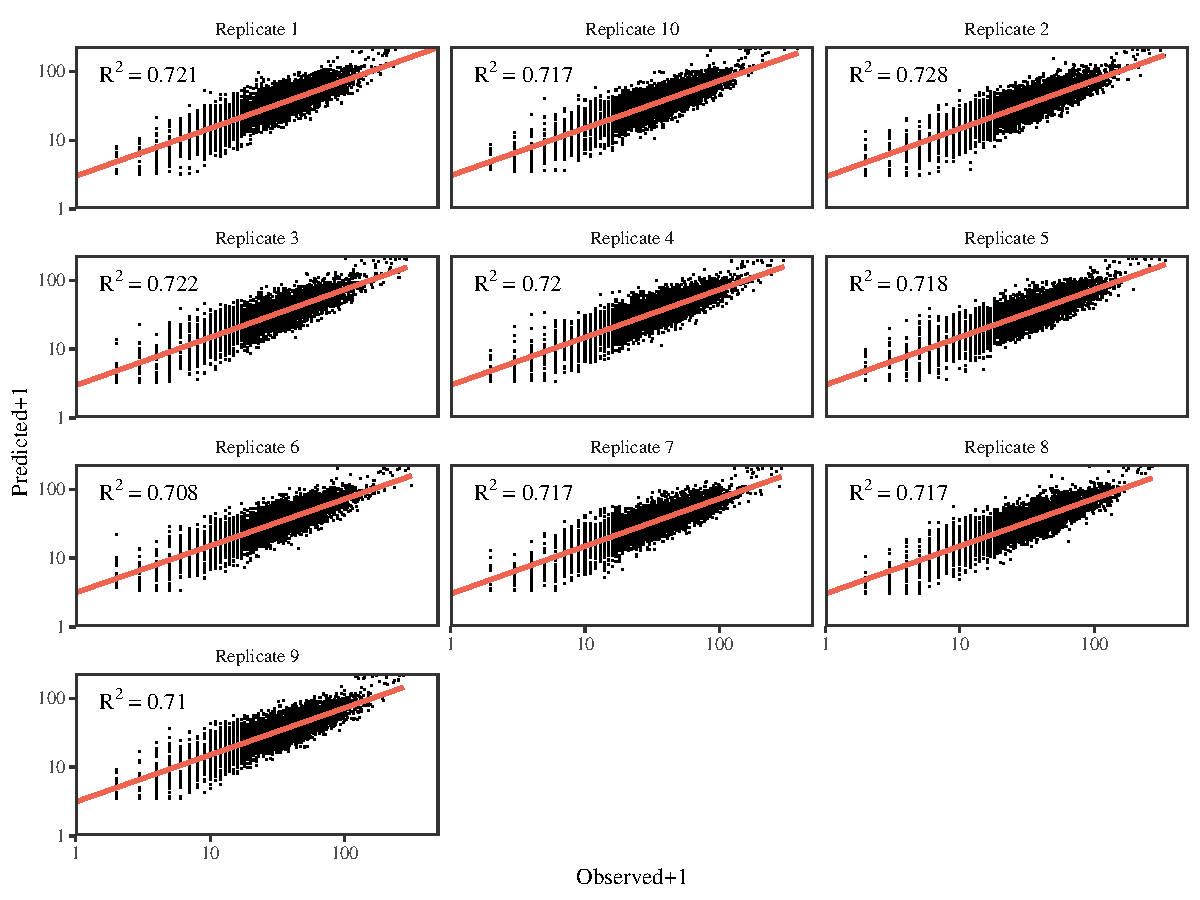
\includegraphics[width=\textwidth]{../figure_rep/figure_stanfit_rep_traj_2.pdf}
\caption{
\textbf{Summary of comparisons between observed and predicted epidemic trajectories from simulation recovery experiments.}
}
\end{figure}

\pagebreak

\begin{figure}[!ht]
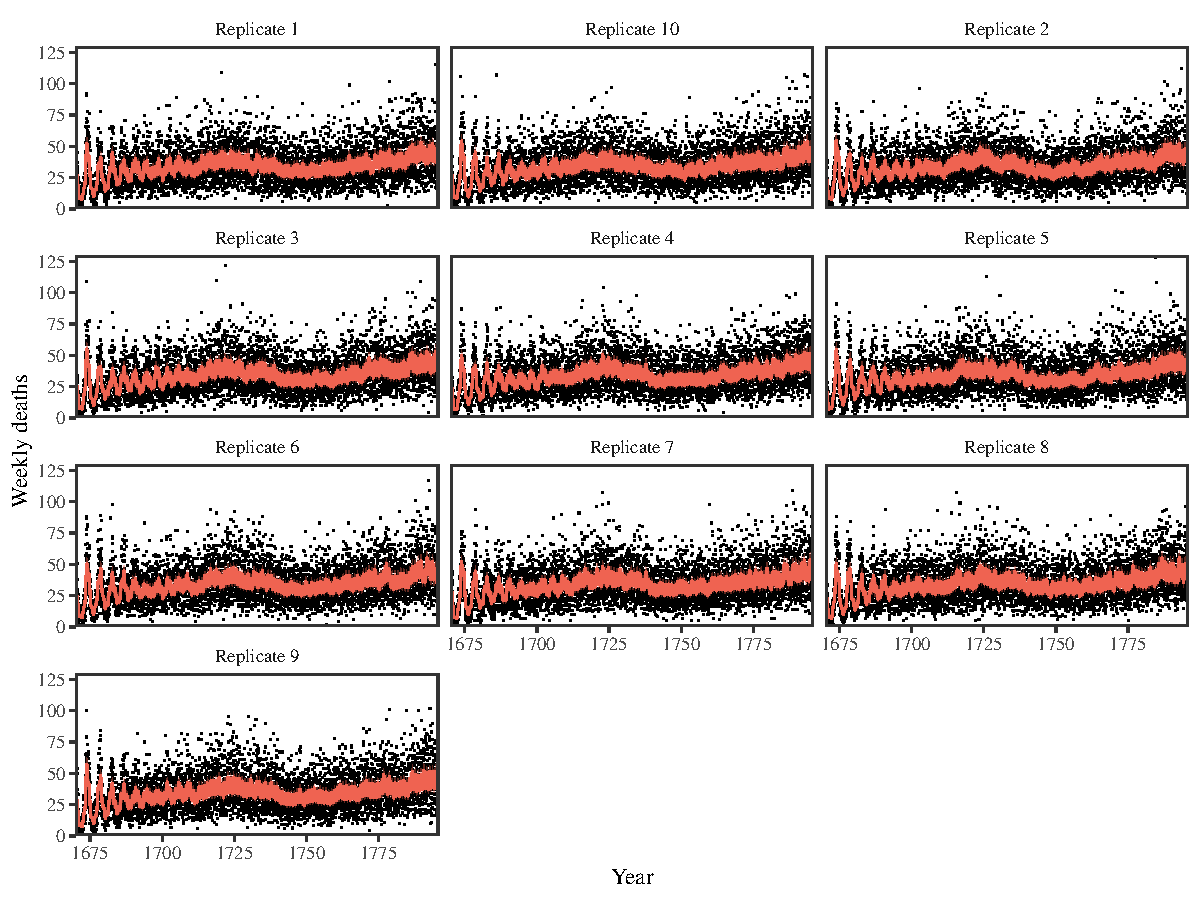
\includegraphics[width=\textwidth]{../figure_rep_nc/figure_stanfit_rep_traj_1.pdf}
\caption{
\textbf{Comparisons between observed and predicted epidemic trajectories from simulation recovery experiments in the absence of long-term changes in transmission.}
}
\end{figure}

\pagebreak


\begin{figure}[!ht]
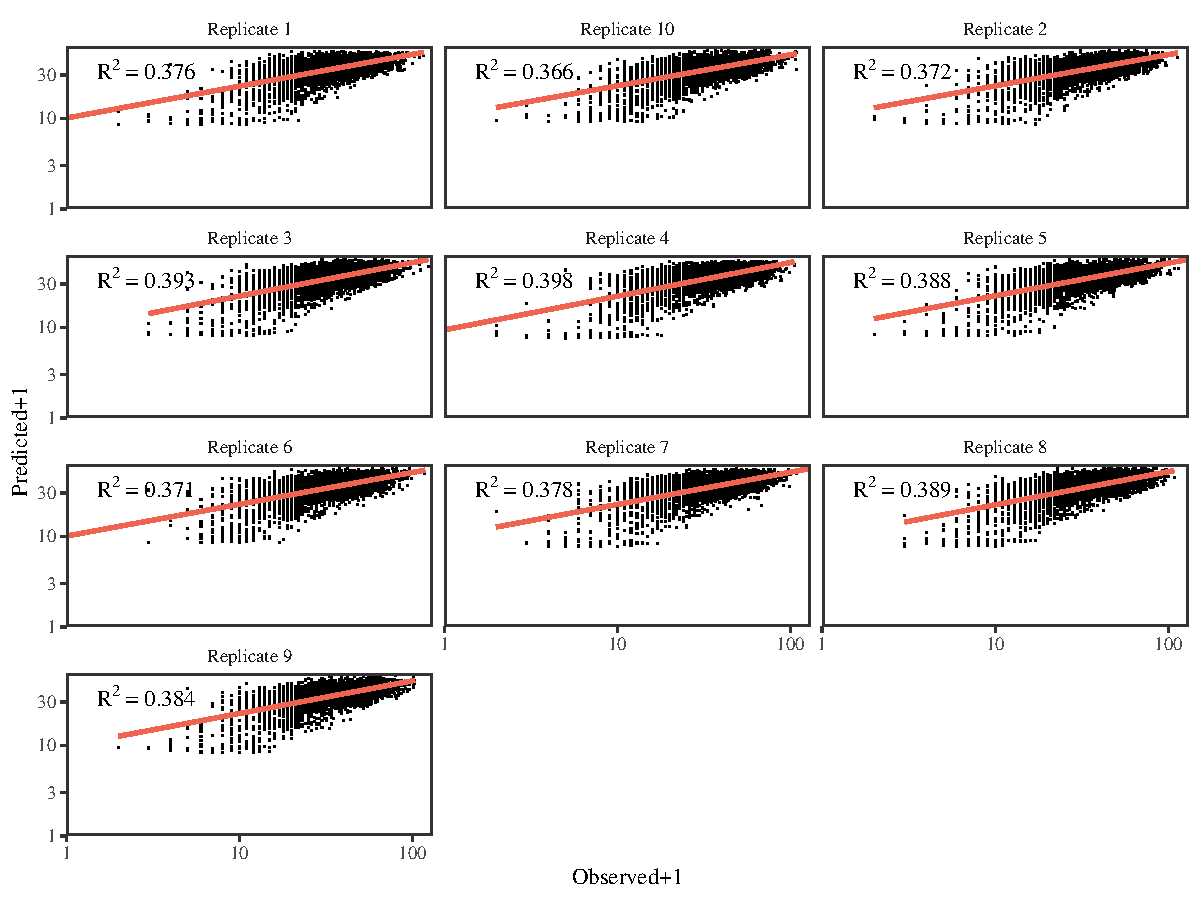
\includegraphics[width=\textwidth]{../figure_rep_nc/figure_stanfit_rep_traj_2.pdf}
\caption{
\textbf{Summary of comparisons between observed and predicted epidemic trajectories from simulation recovery experiments in the absence of long-term changes in transmission.}
}
\end{figure}


\bibliography{semi-mechanistic}

\end{document}
